\documentclass[t,dvipsnames]{beamer}

\setbeamertemplate{navigation symbols}{}
\useinnertheme{circles}
% \usecolortheme{crane}

% \usepackage[T1]{fontenc}
\usepackage[utf8]{inputenc}
% \usepackage[polish]{babel}
\usepackage[british]{babel}

\usepackage[adobe-utopia]{mathdesign}
\usepackage[series=z]{libgreek}
\usepackage{tgpagella}
\usepackage[textwidth=4cm]{todonotes}
\usepackage{minted}
\usemintedstyle{colorful}
% \usemintedstyle{autumn}
% \usemintedstyle{vs}
\usepackage{tikz}
\usetikzlibrary{matrix,arrows,calc}
\tikzset{every scope/.style={>=angle 60,thick}}

\author{Marcin Szamotulski}
\institute{\insertlogo{
\includegraphics[height=0.4cm]{iohk-logo.png}}}
\title{Free Categories and State Machines}

\setbeamertemplate{frametitle}[default][center]

\begin{document}
\begin{frame}
    \titlepage
\end{frame}

\begin{frame}[fragile]
    \frametitle{\underline{Monoids}}
    \framesubtitle{Categories with a single object}
    \begin{columns}[t]
        \begin{column}{0.5\textwidth}
            \begin{minted}[stripall,bgcolor=NavyBlue!5!white,fontsize=\tiny]{haskell}
class Semigroup s where
  -- prop> a <> (b <> c) = (a <> b) <> c
  (<>) :: s -> s -> s

class Semigroup m => Monoid m where
  -- prop> a <> unit = a = unit <> a
  unit = m

data MonoidAsCategory
       m (k :: ()) (k' :: ())
       where
  MonoidAsCategory
    :: m
    -> MonoidAsCategory m '() '()

instance Monoid m
      => Category (MonoidAsCategory m)
      where
    id :: forall m (a :: ()).
          Monoid m
       => MonoidAsCategory m a a
    id = unsafeCoerce
          (MonoidAsCategory (unit :: m))

    (MonoidAsCategory x)
       . (MonoidAsCategory y)
       = MonoidAsCategory (x <> y)

            \end{minted}
        \end{column}
        \begin{column}{0.5\textwidth}
          \begin{minted}[stripall,bgcolor=NavyBlue!5!white,fontsize=\tiny]{haskell}
class Category (c :: k -> k -> *) where
  -- prop> id . f = f = f . id
  id  :: c x x
  -- prop> f . (g . h) = (f . g) .h
  (.) :: c y z
      -> c x y
      -> c x z
            \end{minted}
            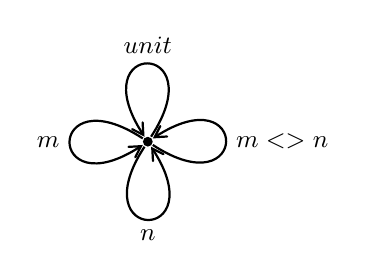
\begin{tikzpicture}
              \node[fill,inner sep=1.25pt,circle] (O) {};
              \draw[->]            (O) .. controls +(0.85,1.3) and +(-0.85,1.3).. (O) node[above,pos=0.5]{\small{$unit$}};
              \draw[->,rotate=90]  (O) .. controls +(0.85,1.3) and +(-0.85,1.3).. (O) node[left, pos=0.5]{\small{$m$}};
              \draw[->,rotate=180] (O) .. controls +(0.85,1.3) and +(-0.85,1.3).. (O) node[below,pos=0.5]{\small{$n$}};
              \draw[->,rotate=270] (O) .. controls +(0.85,1.3) and +(-0.85,1.3).. (O) node[right,pos=0.5]{\small{$m <> n$}};
            \end{tikzpicture}
        \end{column}
    \end{columns}
\end{frame}

\begin{frame}[fragile]
  \frametitle{\underline{Categories}}
  \framesubtitle{Monoids with many objects}
  \begin{minted}[stripall,bgcolor=NavyBlue!5!white,fontsize=\tiny]{haskell}
class Category (c :: k -> k -> *) where
  -- prop> id . f = f = f . id
  id  :: c x x
  -- prop> f . (g . h) = (f . g) .h
  (.) :: c y z
      -> c x y
      -> c x z

instance Category c
      => Monoid (c a a)
      where
  unit = id
  x <> y = x . y
  \end{minted}
  \vspace{-20pt}
  \begin{center}
    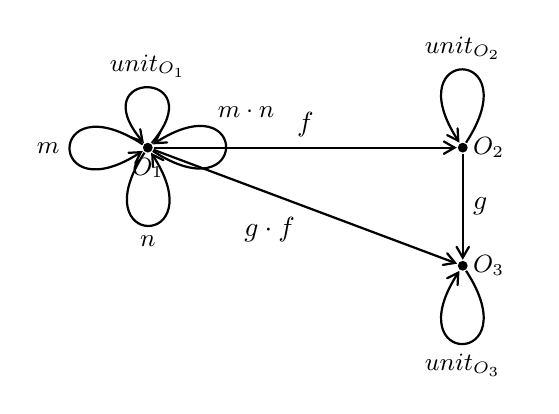
\begin{tikzpicture}
      \node[fill,inner sep=1.25pt,circle] (O1) at (0, 0) {};
      \node[below] at (O1) {\small{$O_1$}};
      \node[fill,inner sep=1.25pt,circle] (O2) at (4, 0) {};
      \node[right] at (O2) {\small{$O_2$}};
      \node[fill,inner sep=1.25pt,circle] (O3) at (4, -1.5) {};
      \node[right] at (O3) {\small{$O_3$}};
      \draw[->]            (O1) .. controls +(0.85,1)   and +(-0.85,1)   .. (O1) node[above,      pos=0.5] {\small{$unit_{O_1}$}};
      \draw[->,rotate=90]  (O1) .. controls +(0.85,1.3) and +(-0.85,1.3) .. (O1) node[left,       pos=0.5] {\small{$m$}};
      \draw[->,rotate=180] (O1) .. controls +(0.85,1.3) and +(-0.85,1.3) .. (O1) node[below,      pos=0.5] {\small{$n$}};
      \draw[->,rotate=270] (O1) .. controls +(0.85,1.3) and +(-0.85,1.3) .. (O1) node[above right,pos=0.75]{\small{$m \cdot n$}};
      \draw[->] (O2) .. controls +(0.85,1.3)  and +(-0.85, 1.3)  .. (O2) node[above,pos=0.5]{\small{$unit_{O_2}$}};
      \draw[->] (O3) .. controls +(0.85,-1.3) and +(-0.85, -1.3) .. (O3) node[below,pos=0.5]{\small{$unit_{O_3}$}};
      \draw[->] (O1) -- (O2) node[above,pos=0.5]{$f$};
      \draw[->] (O2) -- (O3) node[right,pos=0.5]{$g$};
      \draw[->] (O1) -- (O3) node[below left,pos=0.5]{$g\cdot f$};
    \end{tikzpicture}
  \end{center}
\end{frame}

\begin{frame}[fragile]
  \frametitle{Examples}
  Any set is a (discrete) category
  \begin{center}
    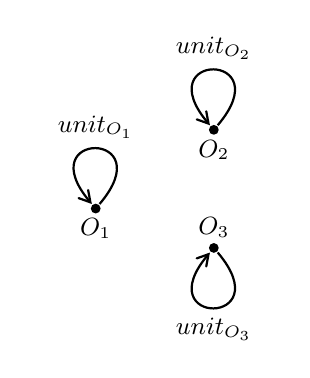
\begin{tikzpicture}
      \node[fill,inner sep=1.25pt,circle] (O1) at (0, 0) {};
      \node[below] at (O1) {\small{$O_1$}};
      \node[fill,inner sep=1.25pt,circle] (O2) at (1.5, 1) {};
      \node[below] at (O2) {\small{$O_2$}};
      \node[fill,inner sep=1.25pt,circle] (O3) at (1.5, -0.5) {};
      \node[above] at (O3) {\small{$O_3$}};
      \draw[->] (O1) .. controls +(0.85,1) and +(-0.85,1)   .. (O1) node[above, pos=0.5] {\small{$unit_{O_1}$}};
      \draw[->] (O2) .. controls +(0.85,1) and +(-0.85,1)   .. (O2) node[above, pos=0.5] {\small{$unit_{O_2}$}};
      \draw[->] (O3) .. controls +(0.85,-1) and +(-0.85,-1) .. (O3) node[below, pos=0.5] {\small{$unit_{O_3}$}};
    \end{tikzpicture}
  \end{center}
  \hline
  \vspace{5}
  Natural numbers
  \begin{center}
    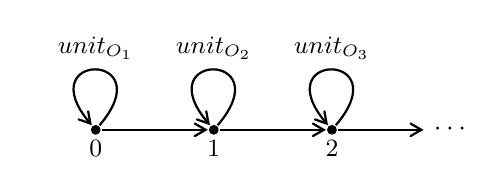
\begin{tikzpicture}
      \node[fill,inner sep=1.25pt,circle] (O0) at (0, 0) {};
      \node[below] at (O0) {\small{$0$}};
      \node[fill,inner sep=1.25pt,circle] (O1) at (1.5, 0) {};
      \node[below] at (O1) {\small{$1$}};
      \node[fill,inner sep=1.25pt,circle] (O2) at (3, 0) {};
      \node[below] at (O2) {\small{$2$}};
      \node (O3) at (4.5, 0) {$\cdots$};
      \draw[->] (O0) .. controls +(0.85,1) and +(-0.85,1)   .. (O0) node[above, pos=0.5] {\small{$unit_{O_1}$}};
      \draw[->] (O0) -- (O1);
      \draw[->] (O1) .. controls +(0.85,1) and +(-0.85,1)   .. (O1) node[above, pos=0.5] {\small{$unit_{O_2}$}};
      \draw[->] (O1) -- (O2);
      \draw[->] (O2) .. controls +(0.85,1) and +(-0.85,1)   .. (O2) node[above, pos=0.5] {\small{$unit_{O_3}$}};
      \draw[->] (O2) -- (O3);
    \end{tikzpicture}
  \end{center}
\end{frame}

\begin{frame}[fragile,c]
  \frametitle{Examples}
  \begin{center}
    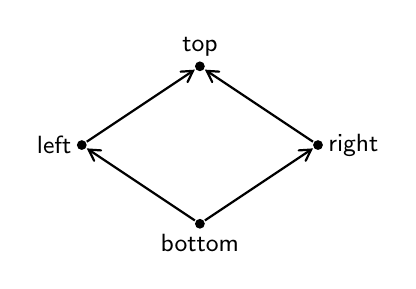
\begin{tikzpicture}
      \node[fill,inner sep=1.25pt,circle] (O0) at (0, 0) {};
      \node[below] at (O0) {\sf\small{bottom}};
      \node[fill,inner sep=1.25pt,circle] (O1) at (-1.5, 1) {};
      \node[left] at (O1) {\sf\small{left}};
      \node[fill,inner sep=1.25pt,circle] (O2) at (1.5, 1) {};
      \node[right] at (O2) {\sf\small{right}};
      \node[fill,inner sep=1.25pt,circle] (O3) at (0, 2) {};
      \node[above] at (O3) {\sf\small{top}};

      \draw[->] (O0) -- (O1);
      \draw[->] (O0) -- (O2);
      \draw[->] (O1) -- (O3);
      \draw[->] (O2) -- (O3);
    \end{tikzpicture}
  \end{center}
\end{frame}

\begin{frame}[fragile]
    \frametitle{\underline{Free Algebras}}
    \begin{minted}[stripall,bgcolor=NavyBlue!5!white,fontsize=\tiny]{haskell}
type family AlgebraType  (f :: k) (a :: l) :: Constraint
type family AlgebraType0 (f :: k) (a :: l) :: Constraint

data Proof (c :: Constraint) (a :: l) where
    Proof :: c => Proof c a

class FreeAlgebra (m :: Type -> Type)  where
    returnFree :: a -> m a

    foldMapFree
        :: forall d a.
         ( AlgebraType  m d
         , AlgebraType0 m a
         )
        =>   (a -> d) -- ^ a map generators into @d@
        -> (m a -> d) -- ^ a homomorphism from @m a@ to @d@

    codom  :: forall a. AlgebraType0 m a => Proof (AlgebraType m (m a)) (m a)

    default codom :: forall a. AlgebraType m (m a)
                  => Proof (AlgebraType m (m a)) (m a)
    codom = Proof

    forget :: forall a. AlgebraType  m a => Proof (AlgebraType0 m a) (m a)

    default forget :: forall a. AlgebraType0 m a
                   => Proof (AlgebraType0 m a) (m a)
    forget = Proof

    \end{minted}
\end{frame}

\begin{frame}[fragile]
    \frametitle{\underline{Free Semigroups and Monoids}}
    % \framesubtitle{sequences}
    \begin{minted}[stripall,bgcolor=NavyBlue!5!white,fontsize=\tiny]{haskell}
type instance AlgebraType0 NonEmpty a = ()
type instance AlgebraType  NonEmpty m = Semigroup m
instance FreeAlgebra NonEmpty where
    returnFree a = a :| []
    foldMapFree f (a :| []) = f a
    foldMapFree f (a :| (b : bs)) = f a <> foldMapFree f (b :| bs)

instance Semigroup [a] where
  -- (<>) = (++) _concatenation_
  (x : xs) <> ys = x : (xs <> ys)
  []       <> ys = ys
    \end{minted}

    \begin{minted}[stripall,bgcolor=NavyBlue!5!white,fontsize=\tiny]{haskell}
instance Monoid [a] where
  unit = []

type instance AlgebraType [] m = Monoid m
instance FreeAlgebra [] where
    returnFree a = [a]
    -- foldMapFree = foldMap
    foldMapFree _ [] = unit
    foldMapFree f (a : as) = f a <> foldMapFree f as

    \end{minted}
\end{frame}

\begin{frame}[c]
  \frametitle{\underline{Why Free Algebras are Important?}}
  \begin{itemize}
    \item A free algebra can be interpreted in any other algebra (of the same
    type). e.g.\\[10pt]
        \begin{itemize}
          \item given \mintinline{haskell}{f :: Monoid d => a -> d} we have
            a monoid homomorphism
                \mintinline{haskell}{foldMap f :: Monoid d => [a] ->
                d}.\\[10pt]
          \item given \mintinline{haskell}{f :: Semigroup d => a -> d}
            we can construct a semigroup homorphism
            \mintinline{haskell}{Semigroup d => NonEmpty a -> d}\\[10pt]
          \item given \mintinline{haskell}{f :: Monad m => (forall x. f x ->
            m x)} we have monad morphism
            \mintinline{haskell}{foldFree f :: Monad m => Free f a -> m a}
        \end{itemize}
  \end{itemize}
\end{frame}
\begin{frame}
  \frametitle{\underline{Why Free Algebras are Important?}}
  \begin{itemize}
    \item Birhoff's Theorem!
      \begin{theorem}[G.Birkhoff 1935]
        Every variety is an equational theory.
      \end{theorem}
      \begin{itemize}
        \item Why this is important?  Because the proof constructs free
          algebras to show that varieties are equational theories.\\[10pt]
        \item It explains \it{constructively} why semigroups, monoids, Boolean
          or Heyting algebras have free algebras.
      \end{itemize}
  \end{itemize}
\end{frame}

\begin{frame}[fragile]
  \frametitle{\underline{Higher Kinded Free Algebras}}
  \begin{minted}[stripall,bgcolor=NavyBlue!5!white,fontsize=\tiny]{haskell}
class FreeAlgebra2 (m :: (k -> k -> Type) -> k -> k -> Type) where
  liftFree2    :: f a b
               -> m f a b

  foldNatFree2 :: forall (d :: k -> k -> Type)
                         (f :: k -> k -> Type) a b .
                  ( AlgebraType  m d
                  , AlgebraType0 m f
                  )
               => (forall x y. f x y -> d x y)
               -> (m f a b -> d a b)

  codom2  :: forall (f :: k -> k -> Type).
             AlgebraType0 m f
          => Proof (AlgebraType m (m f)) (m f)

  default codom2 :: forall a. AlgebraType m (m a)
                 => Proof (AlgebraType m (m a)) (m a)
  codom2 = Proof

  forget2 :: forall (f :: k -> k -> Type).
             AlgebraType m f
          => Proof (AlgebraType0 m f) (m f)

  default forget2 :: forall a. AlgebraType0 m a
                  => Proof (AlgebraType0 m a) (m a)
  forget2 = Proof
  \end{minted}
\end{frame}

\begin{frame}[fragile]
  \frametitle{\underline{Free Categories}}
  \framesubtitle{type aligned sequences}
  \begin{minted}[stripall,bgcolor=NavyBlue!5!white,fontsize=\tiny]{haskell}
data ListTr :: (k -> k -> *) -> k -> k -> * where
  NilTr  :: ListTr f a a
  ConsTr :: f b c -> ListTr f a b -> ListTr f a c

instance Category ListTr where
  id = NilTr
  -- concatenation
  (ConsTr x xs) . ys = ConsTr x (xs . ys)
  NilTr         . ys = ys

type instance AlgebraType  ListTr c = Category c
instance FreeAlgebra2 ListTr where
  liftFree2 a  = ListTr a NilTr
  foldNatFree2 _   NilTr          = id
  foldNatFree2 fun (ConsTr bc ab) = fun bc . foldNatFree2 fun ab
  \end{minted}

  \only<2->{
  There are other possible representations:
  \begin{itemize}
      \item Okasaki's realtime queues
      \item Church encoding
      \item ...
  \end{itemize}
  \sf{Benchmarks:} \url{https://coot.me/bench-cats.html}}
\end{frame}

\begin{frame}[fragile]
    \frametitle{\underline{Kleisli categories}}
    \framesubtitle{... and beyond}
    \vspace{1em}
    \begin{minted}[stripall,bgcolor=NavyBlue!5!white,fontsize=\tiny]{haskell}
newtype Kleisli m a b = Kleisli { runKleisli :: a -> m b }

instance Monad m => Category (Kleisli m) where
    id = Kleisli return
    -- (.) ~ (>=>)
    (Kleisli f) . (Kleisli g) = Kleisli (\x -> g x >>= f)
    \end{minted}

    % morally a title
    \center{\usebeamercolor[fg]{frametitle}\large\underline{Effectful Categories}}
    \begin{minted}[stripall,bgcolor=NavyBlue!5!white,fontsize=\tiny]{haskell}
-- | Categories which can lift monadic actions.
--
class Category c => EffectCategory c m | c -> m where
  effect :: m (c a b) -> c a b

instance Monad m => EffectCategory (Kleisli m) m where
  effect m = Kleisli (\a -> m >>= \(Kleisli f) -> f a)

instance EffectCategory (->) Identity where
  effect = runIdentity
    \end{minted}
\end{frame}

\begin{frame}[fragile]
    \frametitle{\underline{Free Effectful Categories}}
    \begin{minted}[stripall,bgcolor=NavyBlue!5!white,fontsize=\tiny]{haskell}
-- | Category transformer, which adds @'EffectCategory'@ instance to the
-- underlying base category.
--
data EffCat :: (* -> *) -> (k -> k -> *) -> k -> k -> * where
  Base   :: c a b -> EffCat m c a b
  Effect :: m (EffCat m c a b) -> EffCat m c a b

instance (Functor m, Category c) => Category (EffCat m c) where
  id = Base id
  Base f    . Base g    = Base   (f . g)
  f         . Effect mg = Effect ((f .) <$> mg)
  Effect mf . g         = Effect ((. g) <$> mf)

instance (Functor m, Category c) => EffectCategory (EffCat m c) m where
  effect = Effect

type instance AlgebraType0 (EffCat m) c = (Monad m, Category c)
type instance AlgebraType  (EffCat m) c  = EffectCategory c m
instance Monad m => FreeAlgebra2 (EffCat m) where
  liftFree2 = Base
  foldNatFree2 nat (Base cab)    = nat cab
  foldNatFree2 nat (Effect mcab) = effect (foldNatFree2 nat <$> mcab)
    \end{minted}
\end{frame}

\begin{frame}
  \frametitle{\underline{Example}}
  \vspace{30pt}
  \only<1>
    {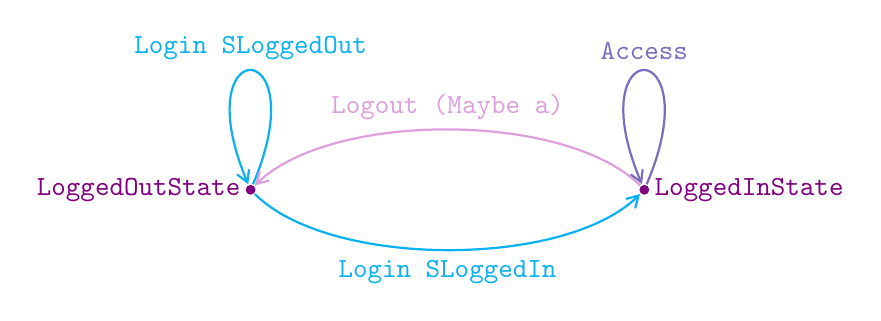
\begin{tikzpicture}
      \node[fill=Purple,inner sep=1.25pt,circle] (LoggedOutState)  at (0, 0) {};
      \node[left,color=Purple] at (LoggedOutState) {\tt{LoggedOutState}};
      \node[fill=Purple,inner sep=1.25pt,circle] (LoggedInState) at (5, 0) {};
      \node[right,color=Purple] at (LoggedInState) {\tt{LoggedInState}};

      \draw[->,color=ProcessBlue]
        (LoggedOutState)
          .. controls +(1,-1) and +(-1,-1)
          .. (LoggedInState)
          node[below,pos=0.5]{\tt{Login\ SLoggedIn}};

      \draw[->, color=ProcessBlue]
        (LoggedOutState)
        .. controls +(0.85,2.0) and +(-0.85,2.0)
        .. (LoggedOutState)
        node[pos=.5,above] {\tt{Login\ SLoggedOut}};

      \draw[<-,color=Plum] (LoggedOutState)
        .. controls +(1,1) and +(-1,1)
        .. (LoggedInState)
        node[above,pos=0.5] {\tt{Logout\ (Maybe a)}};

      \draw[->,color=Periwinkle] (LoggedInState)
        .. controls +(0.85,2.0) and +(-0.85,2.0)
        .. (LoggedInState)
        node[above,pos=0.5] {\tt{Access}};
    \end{tikzpicture}}
  \only<2>{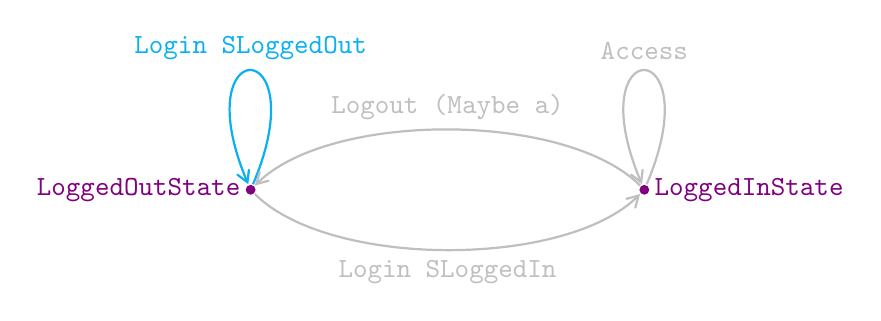
\begin{tikzpicture}
      \node[fill=Purple,inner sep=1.25pt,circle] (LoggedOutState)  at (0, 0) {};
      \node[left,color=Purple] at (LoggedOutState) {\tt{LoggedOutState}};
      \node[fill=Purple,inner sep=1.25pt,circle] (LoggedInState) at (5, 0) {};
      \node[right,color=Purple] at (LoggedInState) {\tt{LoggedInState}};

      \draw[->,color=lightgray]
        (LoggedOutState)
          .. controls +(1,-1) and +(-1,-1)
          .. (LoggedInState)
          node[below,pos=0.5]{\tt{Login\ SLoggedIn}};

      \draw[->, color=ProcessBlue]
        (LoggedOutState)
        .. controls +(0.85,2.0) and +(-0.85,2.0)
        .. (LoggedOutState)
        node[pos=.5,above] {\tt{Login\ SLoggedOut}};

      \draw[<-,color=lightgray] (LoggedOutState)
        .. controls +(1,1) and +(-1,1)
        .. (LoggedInState)
        node[above,pos=0.5] {\tt{Logout\ (Maybe a)}};

      \draw[->,color=lightgray] (LoggedInState)
        .. controls +(0.85,2.0) and +(-0.85,2.0)
        .. (LoggedInState)
        node[above,pos=0.5] {\tt{Access}};
  \end{tikzpicture}}
  \only<3->{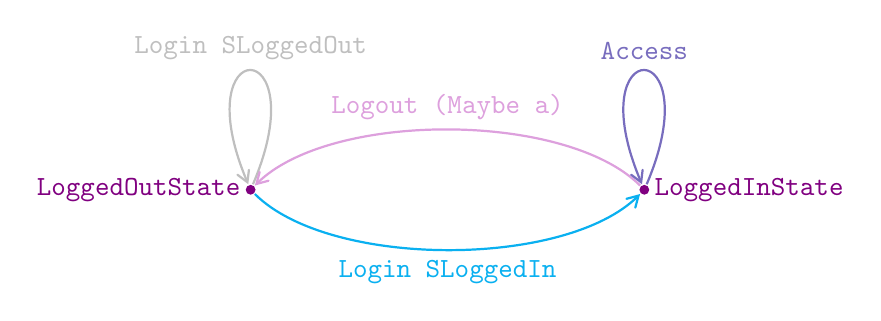
\begin{tikzpicture}
    \node[fill=Purple,inner sep=1.25pt,circle] (LoggedOutState)  at (0, 0) {};
    \node[left,color=Purple] at (LoggedOutState) {\tt{LoggedOutState}};
    \node[fill=Purple,inner sep=1.25pt,circle] (LoggedInState) at (5, 0) {};
    \node[right,color=Purple] at (LoggedInState) {\tt{LoggedInState}};
    \draw[->,color=ProcessBlue]
      (LoggedOutState)
        .. controls +(1,-1) and +(-1,-1)
        .. (LoggedInState)
        node[below,pos=0.5]{\tt{Login\ SLoggedIn}};

    \draw[->, color=lightgray]
      (LoggedOutState)
      .. controls +(0.85,2.0) and +(-0.85,2.0)
      .. (LoggedOutState)
      node[pos=.5,above] {\tt{Login\ SLoggedOut}};

    \draw[<-,color=Plum] (LoggedOutState)
      .. controls +(1,1) and +(-1,1)
      .. (LoggedInState)
      node[above,pos=0.5] {\tt{Logout\ (Maybe a)}};

    \draw[->,color=Periwinkle] (LoggedInState)
      .. controls +(0.85,2.0) and +(-0.85,2.0)
      .. (LoggedInState)
      node[above,pos=0.5] {\tt{Access}};
  \end{tikzpicture}}
  \vspace{10pt}
  \only<4->{\begin{center}
    \url{https://github.com/coot/free-category}\\
    \small{(examples directory)}
  \end{center}}

\end{frame}

\begin{frame}[c]
  \begin{center}
    \textcolor{Purple}{\huge\sf\underline{Thank You!}}
  \end{center}
\end{frame}

\end{document}
